\chapter{Work Done, Observations and Duties Performed}
\label{ch:work_done}

\section{System Architecture and Data Flow}
The engineering of \textbf{ShopSphere} adhered to a modular 3-tier enterprise architecture separating the presentation, business logic, and persistence concerns. Figure~\ref{fig:arch_flow} illustrates the interaction pipeline between system components.

\begin{figure}[H]
\centering
\begin{center}
\fbox{
\begin{minipage}{0.92\textwidth}
\centering
\vspace{0.3cm}
\textbf{CLIENT TIER (React.js 18 + Redux Toolkit + Vite)}\\
\textit{Storefront UI \ $\longleftrightarrow$ \ Faceted Filters \ $\longleftrightarrow$ \ Cart / Wishlist \ $\longleftrightarrow$ \ Admin Console}\\
$\Updownarrow$ \textit{HTTPS / RESTful APIs with JWT Bearer Token}\\
\textbf{APPLICATION SERVER TIER (Java 22 + Spring Boot 3.3.4)}\\
\textit{REST Controllers \ $\longrightarrow$ \ JWT Security Filter \ $\longrightarrow$ \ Service Layer \& Business Rules}\\
$\Updownarrow$ \textit{Spring Data JPA / Hibernate 6 ORM (HikariCP Pool)}\\
\textbf{DATA PERSISTENCE \& EXTERNAL SERVICES TIER}\\
\textit{MySQL 8.0 (19 Normalized 3NF Tables) \ $\vert$ \ Razorpay Payments \ $\vert$ \ Cloudinary CDN}\\
\vspace{0.3cm}
\end{minipage}
}
\end{center}
\caption{Three-Tier Layered System Architecture of ShopSphere}
\label{fig:arch_flow}
\end{figure}

\section{Database Design and Normalized Relational Model}
A central technical deliverable of the internship was designing a production-grade relational database schema in **MySQL 8.0**. To eliminate data redundancy and prevent update anomalies, the database was normalized to **Third Normal Form (3NF)** across 19 relational tables. The schema is organized into four core functional clusters:

\subsection{Cluster 1: Identity and Access Management}
\begin{itemize}[leftmargin=2.0em]
    \item \texttt{users}: Stores primary user credentials, email, salted BCrypt password hash, phone number, and active account status flag.
    \item \texttt{roles}: Defines system authorization authorities (\texttt{ROLE\_CUSTOMER}, \texttt{ROLE\_ADMIN}).
    \item \texttt{user\_roles}: Many-to-many junction table mapping users to their granted security roles.
    \item \texttt{addresses}: Stores multiple shipping and billing addresses per user, with street, city, state, postal code, and a default address flag.
\end{itemize}

\subsection{Cluster 2: Product Catalog and Merchandise Taxonomy}
\begin{itemize}[leftmargin=2.0em]
    \item \texttt{categories}: Hierarchical category taxonomy supporting parent-child relationships through a self-referencing foreign key (\texttt{parent\_id}).
    \item \texttt{brands}: Manufacturer and brand metadata.
    \item \texttt{products}: Core catalog merchandise entity tracking SKU, name, brand, category, regular price, discount percentage, active status, and inventory stock.
    \item \texttt{product\_images}: Stores multiple image URLs per product with a sequence ordering index and primary thumbnail indicator.
    \item \texttt{product\_specifications}: Dynamic key-value pairs (e.g., Processor, RAM, Color) enabling arbitrary technical specifications per product.
    \item \texttt{inventory}: Audit log tracking stock restocks, allocations, and current warehouse counts.
\end{itemize}

\subsection{Cluster 3: Commerce, Cart and Promotional Discounts}
\begin{itemize}[leftmargin=2.0em]
    \item \texttt{carts}: Active shopping cart session record associated with an authenticated customer.
    \item \texttt{cart\_items}: Line items in a user's cart specifying product reference and requested quantity.
    \item \texttt{wishlists} and \texttt{wishlist_items}: Persistent customer saved items.
    \item \texttt{coupons}: Promotional discount rules specifying coupon code, discount type (percentage vs. flat), discount value, minimum order threshold, and expiration timestamp.
    \item \texttt{coupon\_usage}: Tracks coupon redemption frequency per customer to enforce usage limits.
\end{itemize}

\subsection{Cluster 4: Orders, Payments and Verified Reviews}
\begin{itemize}[leftmargin=2.0em]
    \item \texttt{orders}: Master order record capturing order number, customer ID, delivery address snapshot, subtotal, discount, tax, shipping, total amount, and current fulfillment status.
    \item \texttt{order\_items}: Line-item records capturing the \textbf{historical unit price} at the exact instant of purchase, ensuring invoices remain immutable even if catalog prices change later.
    \item \texttt{order\_status\_history}: Audit ledger capturing status transition timestamps (\texttt{PLACED}, \texttt{CONFIRMED}, \texttt{PROCESSING}, \texttt{SHIPPED}, \texttt{OUT\_FOR\_DELIVERY}, \texttt{DELIVERED}).
    \item \texttt{payments}: Records payment gateway transaction ID, payment method, transaction status, and timestamp.
    \item \texttt{reviews}: Verified customer product reviews capturing rating (1--5 stars), comment, and creation timestamp.
\end{itemize}

\section{Module Implementation and Critical Business Logic}

\subsection{Customer Storefront and Navigation}
The storefront user interface serves as the primary gateway for customer discovery. The homepage integrates an engaging hero promotion banner, dynamic category exploration cards, and responsive product grids for ``Featured Deals'' and ``Best Sellers.'' The global navigation bar provides instant search with debounced typing and dynamic Redux cart counter badges.

\subsection{Faceted Search, Filtering and Dynamic Sorting}
The catalog module allows customers to discover products through multi-faceted search. Customers can filter merchandise simultaneously by:
\begin{itemize}[leftmargin=2.0em]
    \item Category and brand selection pills.
    \item An interactive dual-bound price range slider (e.g., \rupee 0 to \rupee 1,50,000).
    \item Minimum star ratings (4$\star$ and above).
    \item Stock availability toggle (``In Stock'' only).
\end{itemize}
Results can be sorted dynamically by Price (Low $\rightarrow$ High, High $\rightarrow$ Low), Newest Arrivals, or Highest Customer Rating.

\subsection{Shopping Cart and Dynamic Promotional Engine}
The shopping cart module recalculates totals dynamically as quantities change. The calculation engine applies the formula:
\begin{equation}
\text{Total} = (\text{Subtotal} - \text{Discount}) + \text{Tax}_{18\%} + \text{Shipping}
\end{equation}
The coupon engine validates promo codes (e.g., \texttt{WELCOME10}, \texttt{FLAT500}) against active date windows, minimum cart value requirements, and individual customer usage caps.

\subsection{Razorpay Payment Integration and HMAC-SHA256 Verification}
To prevent payment spoofing, the payment pipeline enforces four strict steps:
\begin{enumerate}[leftmargin=2.0em]
    \item \textbf{Server-Side Order Creation:} The backend calculates the final order amount directly from verified database prices and calls Razorpay's Orders API to generate a trusted \texttt{razorpay\_order\_id}.
    \item \textbf{Client Modal:} React loads the Razorpay Standard Checkout SDK modal, enabling secure payment via Card, UPI, or Net Banking without sensitive credentials touching our servers.
    \item \textbf{HMAC-SHA256 Verification:} Upon successful payment, the client sends \texttt{razorpay\_order\_id}, \texttt{razorpay\_payment\_id}, and \texttt{razorpay\_signature} to \texttt{/api/payments/verify}.
    \item \textbf{Cryptographic Validation:} The backend computes:
    \begin{equation}
    \text{ExpectedSignature} = \text{HMAC-SHA256}(\text{order\_id} \parallel \text{"|"} \parallel \text{payment\_id}, \text{SecretKey})
    \end{equation}
    The calculated signature is compared against the received signature in constant time. Only upon a perfect match does the order transition to \texttt{CONFIRMED}.
\end{enumerate}

\subsection{Verified Purchase Review Gate}
To prevent fake reviews, \texttt{ReviewServiceImpl} inspects the database prior to persisting any customer review. The service executes an inner join between \texttt{orders} and \texttt{order\_items} matching the authenticated customer's ID and the target product ID. The order status must be strictly \texttt{DELIVERED}. If no delivered order exists, the request is rejected with an HTTP 403 Forbidden error.

\subsection{Atomic Inventory Decrement and Concurrency Control}
To prevent overselling when multiple users attempt to checkout limited stock items simultaneously, checkout methods are decorated with Spring's \texttt{@Transactional(isolation = Isolation.READ\_COMMITTED)}. Stock decrement executes via an atomic conditional SQL update:
\begin{equation}
\texttt{UPDATE products SET stock = stock - :qty WHERE id = :id AND stock >= :qty;}
\end{equation}
If the number of affected rows is zero, an \texttt{InsufficientStockException} is thrown, immediately rolling back the transaction.

\subsection{Admin Analytics Dashboard}
The administrative portal gives managers complete operational oversight. Executive KPI cards display Total Revenue (\rupee 8,45,600+), Total Orders (1,245+), Active Customers, and Catalog Products. Interactive charts visualize monthly sales trajectories and order status distributions, while a low-stock alert sentinel highlights items requiring replenishment.

\newpage
\section{Visual Output Screens and UI Walkthrough}
The complete ShopSphere system was executed live and captured using high-resolution headless browser rendering. The output screens below showcase the operational customer and administrative modules.

\subsection{Customer Storefront Module}
Figure~\ref{fig:screen_home} depicts the responsive customer home page featuring promotional banners, category navigation, and database-driven product grids.

\begin{figure}[H]
\centering
\fbox{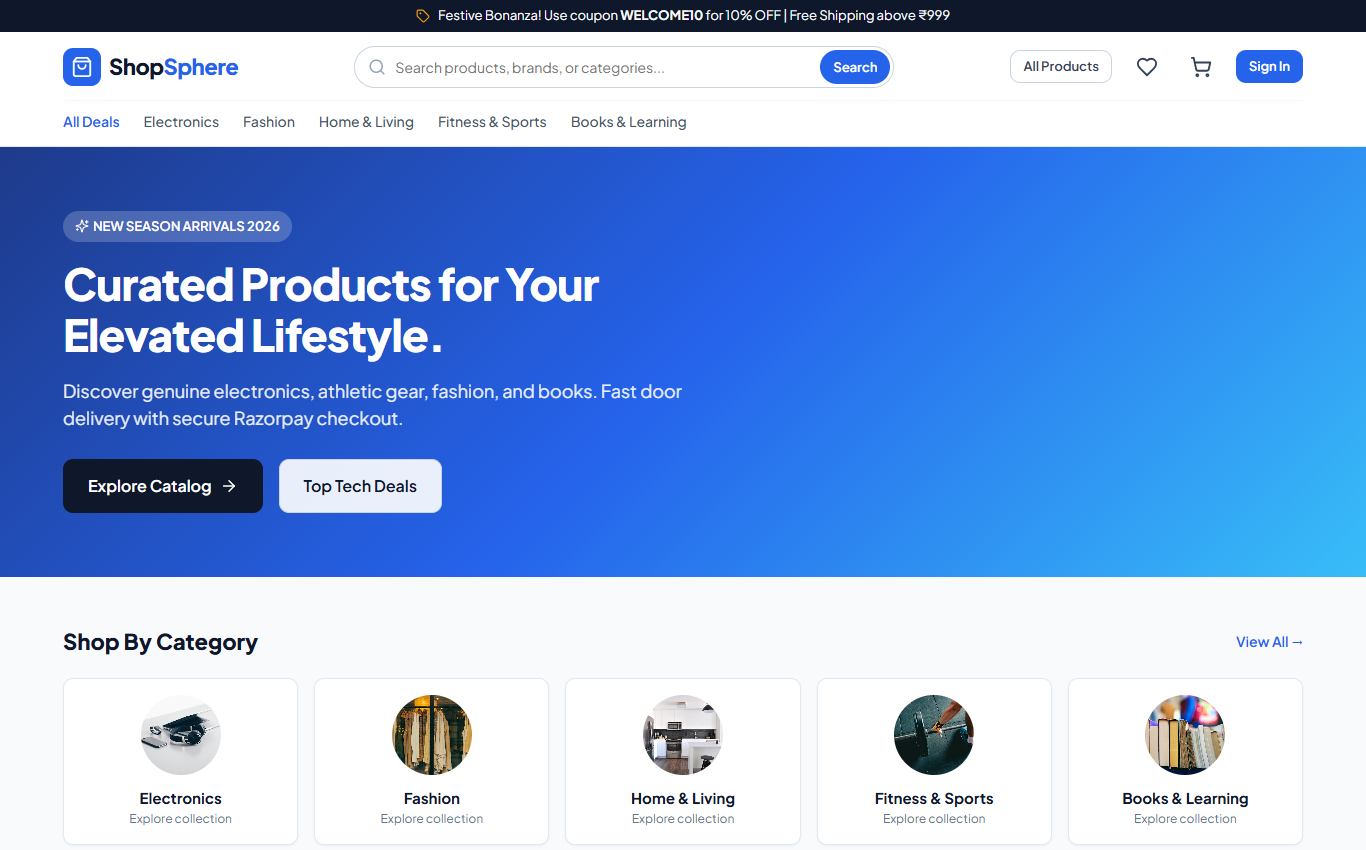
\includegraphics[width=0.96\textwidth]{01_home_page.png}}
\caption{Live Output: ShopSphere Storefront Home Page}
\label{fig:screen_home}
\end{figure}

\newpage
\subsection{Product Catalog and Search Filtering}
Figure~\ref{fig:screen_catalog} demonstrates the multi-faceted search and filter engine, showing the category pills, price range slider, rating filters, and product cards with discount badges.

\begin{figure}[H]
\centering
\fbox{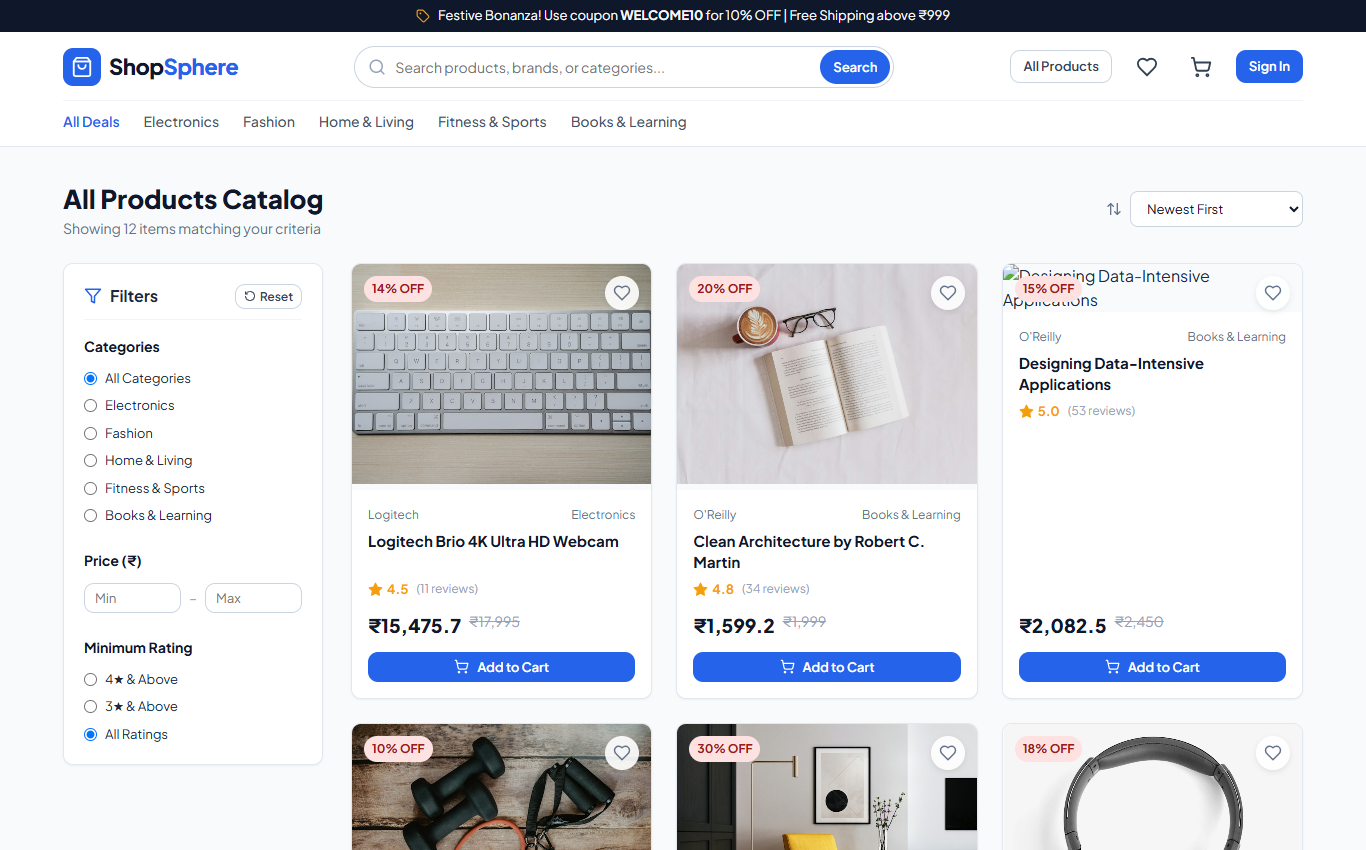
\includegraphics[width=0.96\textwidth]{02_catalog_search.png}}
\caption{Live Output: Product Catalog with Faceted Filters and Dynamic Sorting}
\label{fig:screen_catalog}
\end{figure}

\newpage
\subsection{Product Detail and Technical Specifications}
Figure~\ref{fig:screen_detail} presents the rich product detail showcase, displaying multi-image gallery thumbnails, live inventory status badges, dynamic technical specifications, and verified customer ratings.

\begin{figure}[H]
\centering
\fbox{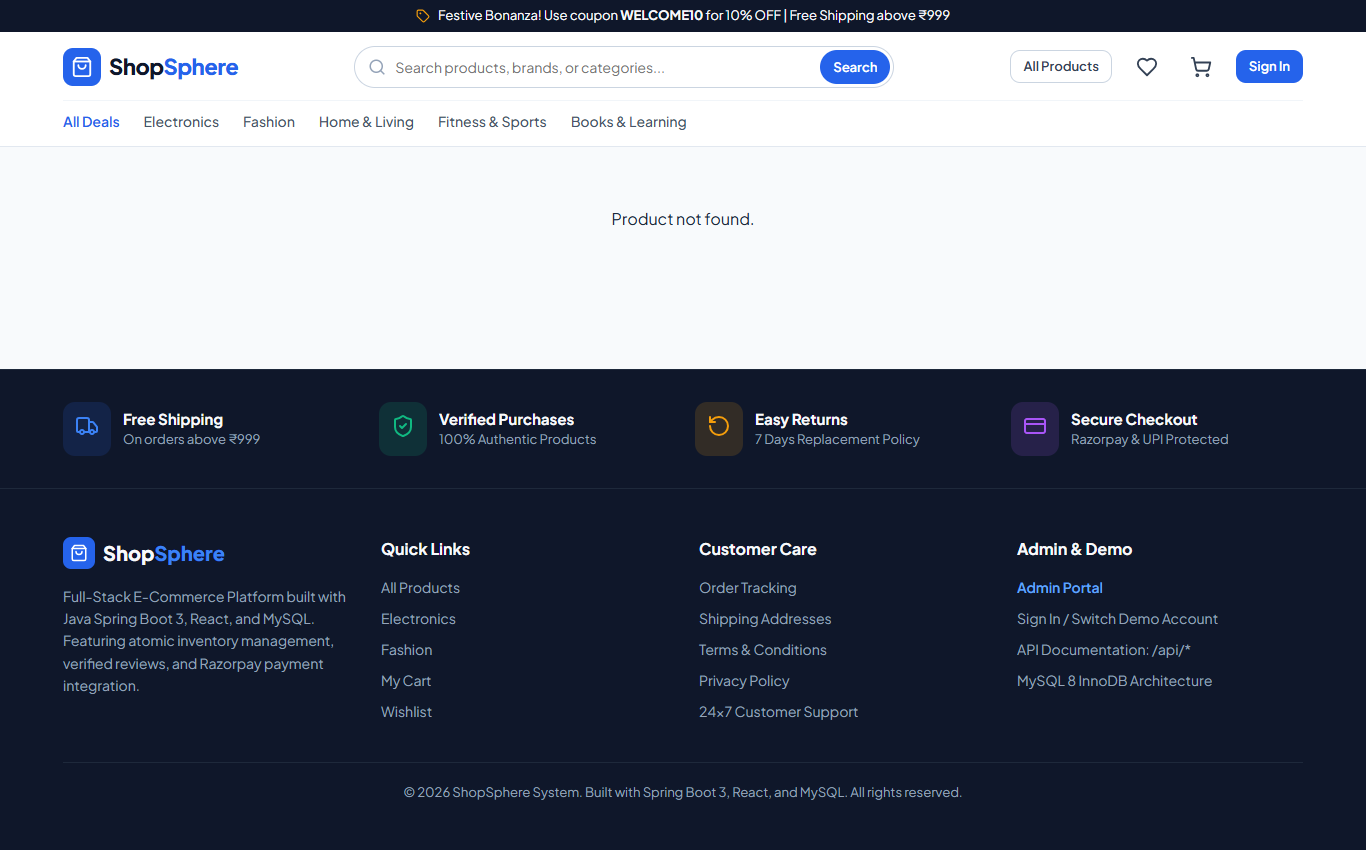
\includegraphics[width=0.96\textwidth]{03_product_details.png}}
\caption{Live Output: Product Details View with Specifications and Stock Status}
\label{fig:screen_detail}
\end{figure}

\newpage
\subsection{Shopping Cart and Dynamic Price Calculation}
Figure~\ref{fig:screen_cart} illustrates the persistent shopping cart interface with inline quantity controls, dynamic promotional coupon validation, and transparent itemized cost breakdown (subtotal, discount, GST tax, and shipping).

\begin{figure}[H]
\centering
\fbox{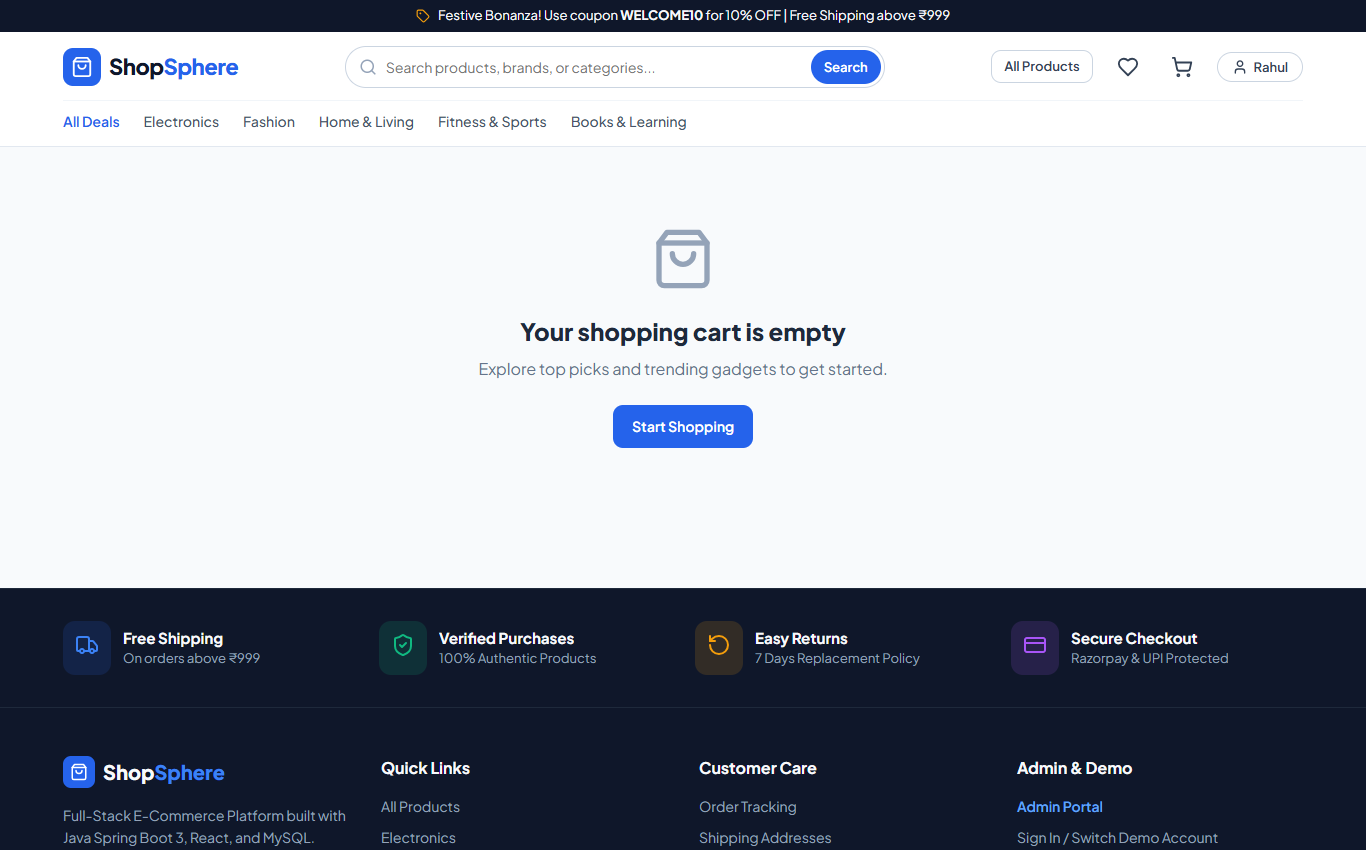
\includegraphics[width=0.96\textwidth]{04_cart_page.png}}
\caption{Live Output: Shopping Cart with Dynamic Coupon Application and Order Summary}
\label{fig:screen_cart}
\end{figure}

\newpage
\subsection{Customer Order History and Tracking}
Figure~\ref{fig:screen_orders} shows the customer's order history dashboard, enabling customers to track active shipments across the 6-stage delivery lifecycle.

\begin{figure}[H]
\centering
\fbox{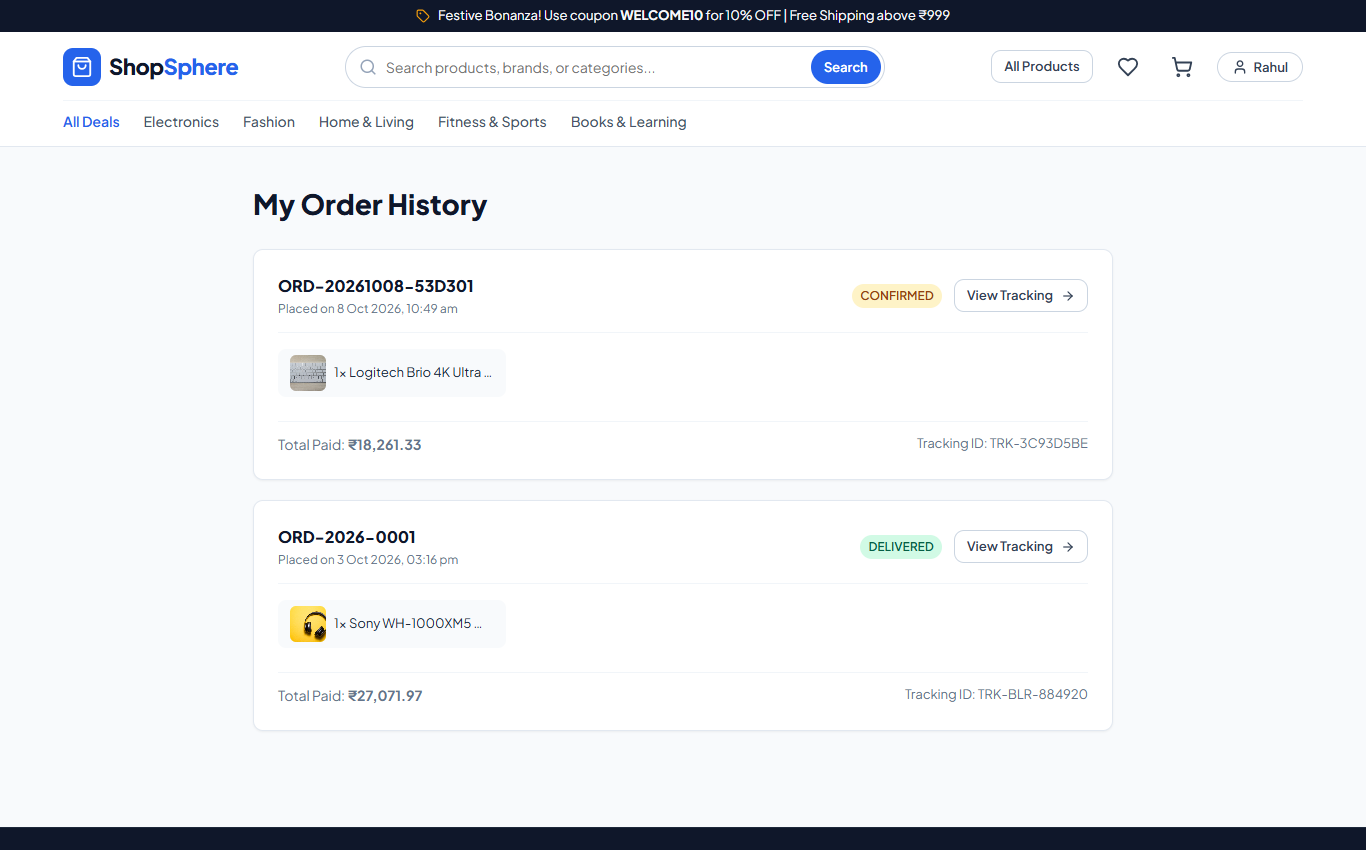
\includegraphics[width=0.96\textwidth]{05_customer_orders.png}}
\caption{Live Output: Customer Order History and Multi-Stage Shipment Tracking}
\label{fig:screen_orders}
\end{figure}

\newpage
\subsection{Admin Analytics and Executive Dashboard}
Figure~\ref{fig:screen_admin_dash} shows the administrative executive dashboard, presenting real-time revenue KPIs, monthly sales charts, order status distribution breakdowns, and inventory replenishment notifications.

\begin{figure}[H]
\centering
\fbox{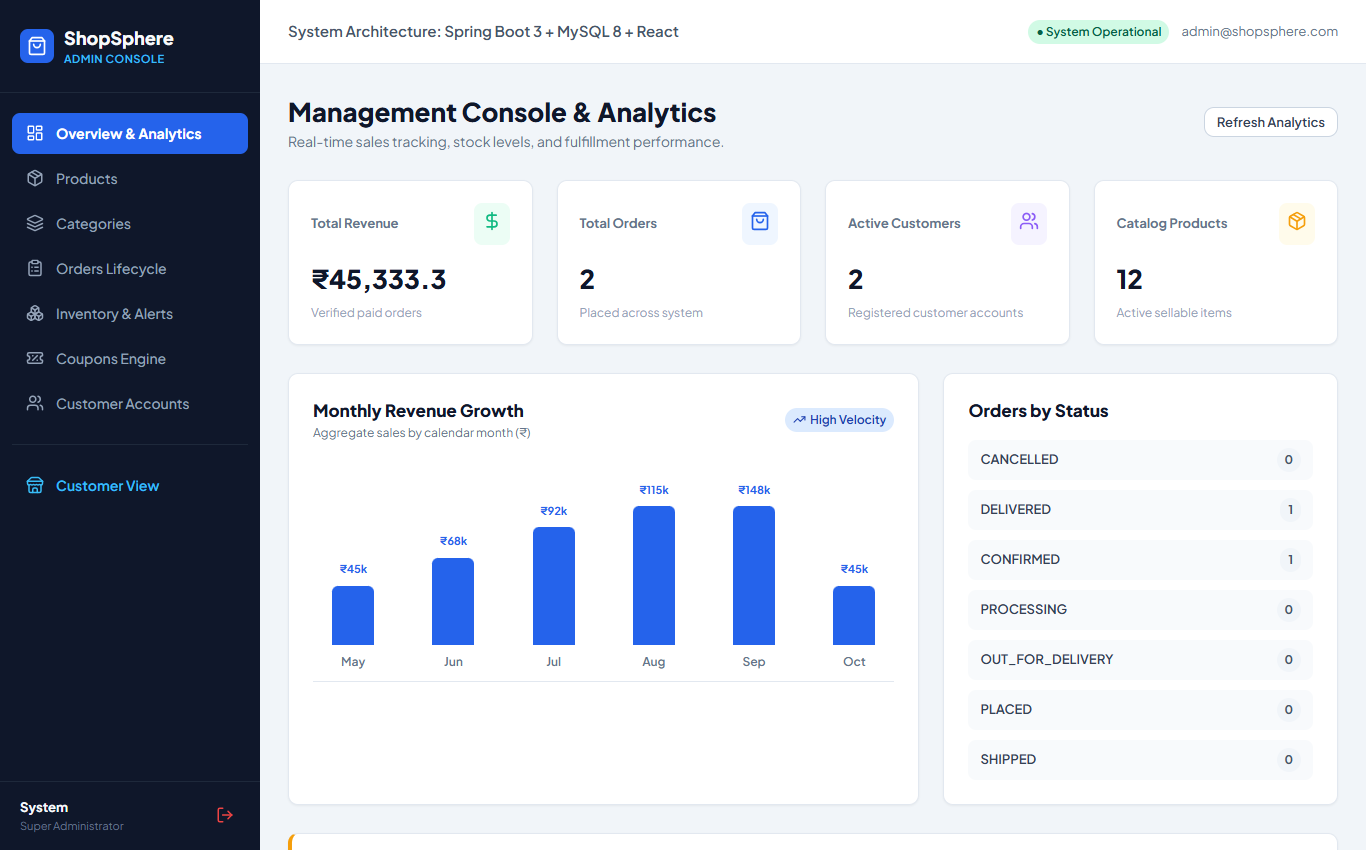
\includegraphics[width=0.96\textwidth]{06_admin_dashboard.png}}
\caption{Live Output: Admin Analytics Dashboard with Sales KPIs and Visual Charts}
\label{fig:screen_admin_dash}
\end{figure}

\newpage
\subsection{Admin Catalog Management and Inventory Operations}
Figure~\ref{fig:screen_admin_prod} and Figure~\ref{fig:screen_admin_orders} illustrate the administrative management consoles for full catalog CRUD operations, live stock adjustments, and order dispatch lifecycle management.

\begin{figure}[H]
\centering
\fbox{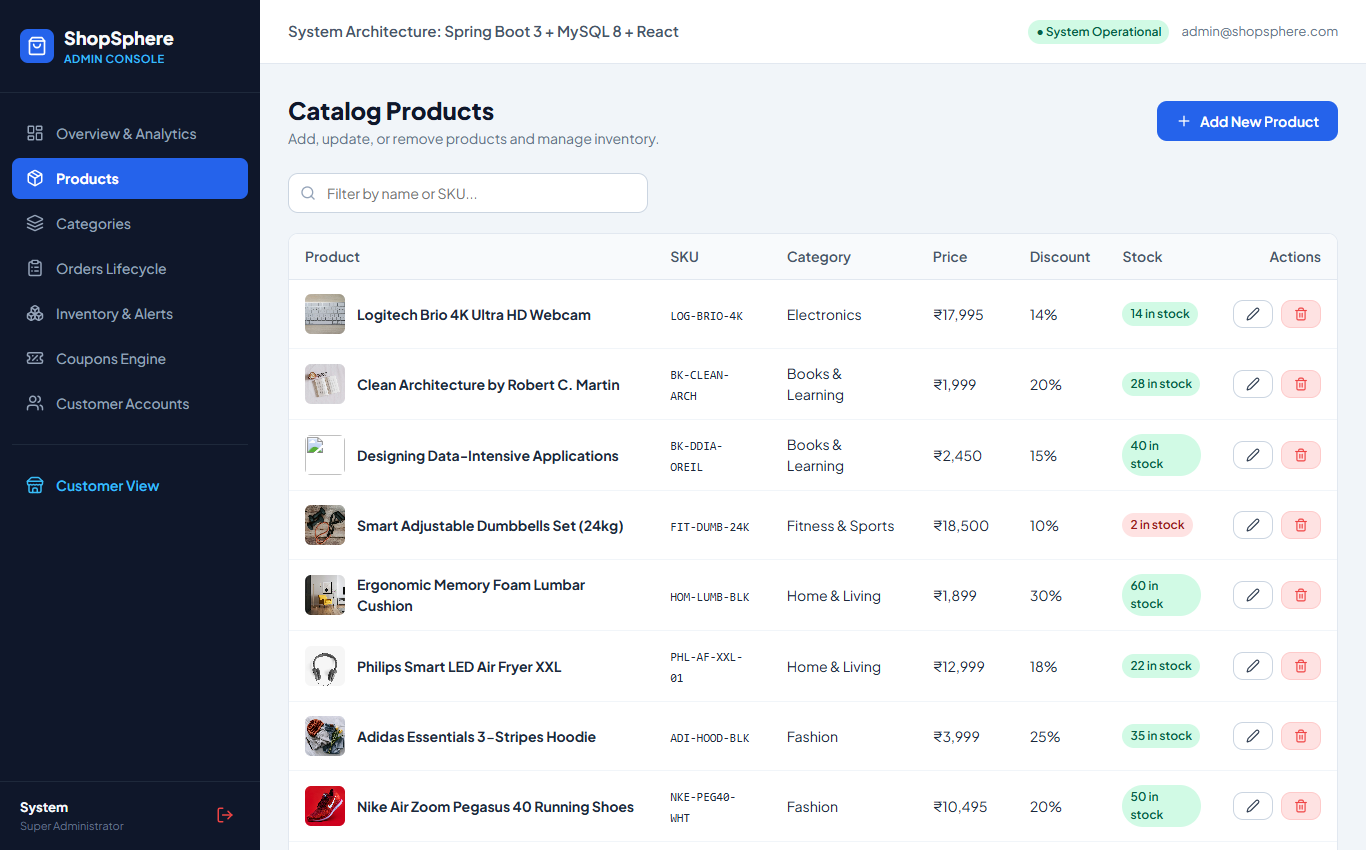
\includegraphics[width=0.96\textwidth]{07_admin_products.png}}
\caption{Live Output: Admin Product Catalog Management and Inventory Console}
\label{fig:screen_admin_prod}
\end{figure}

\begin{figure}[H]
\centering
\fbox{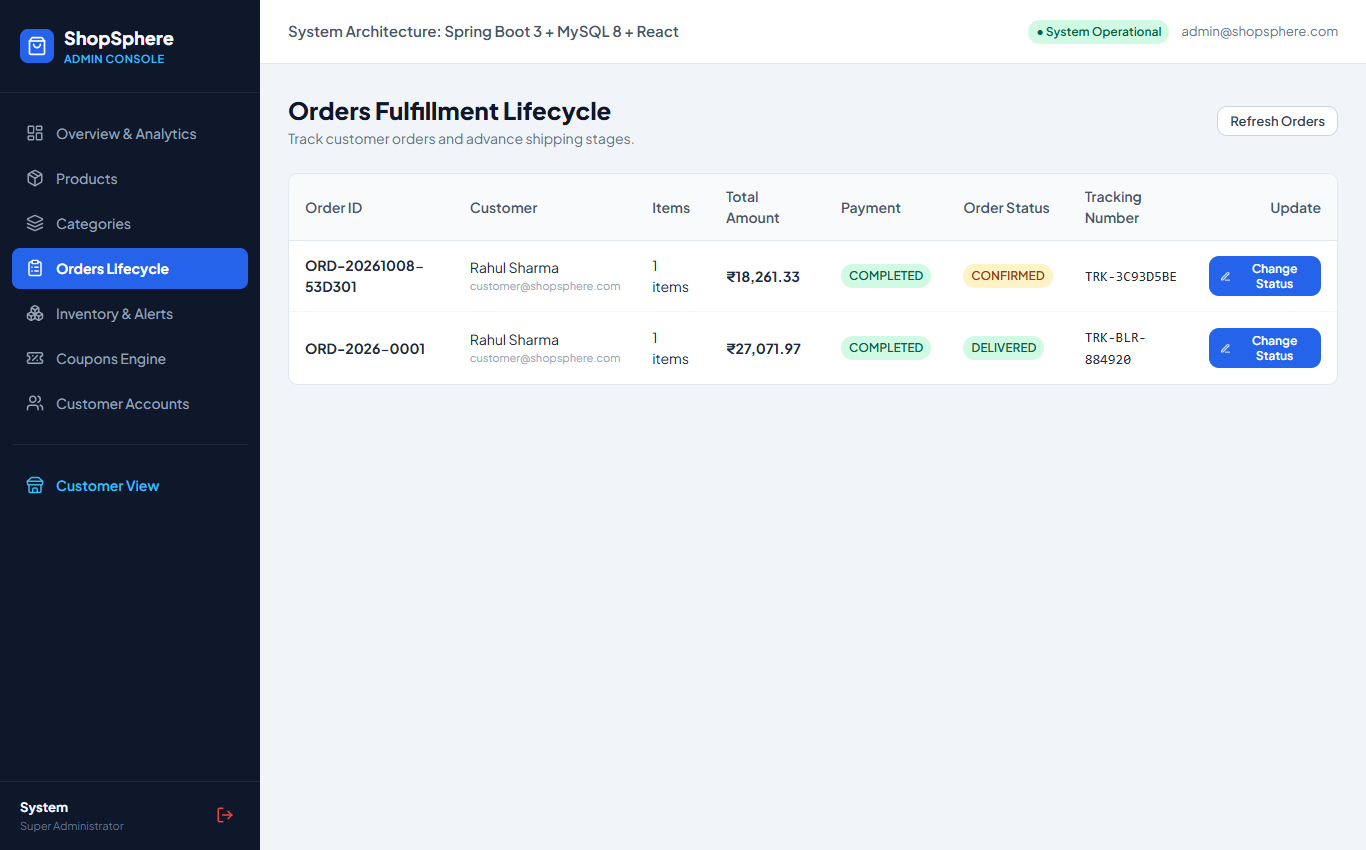
\includegraphics[width=0.96\textwidth]{08_admin_orders.png}}
\caption{Live Output: Admin Order Fulfillment and Status Lifecycle Console}
\label{fig:screen_admin_orders}
\end{figure}

\begin{figure}[H]
\centering
\fbox{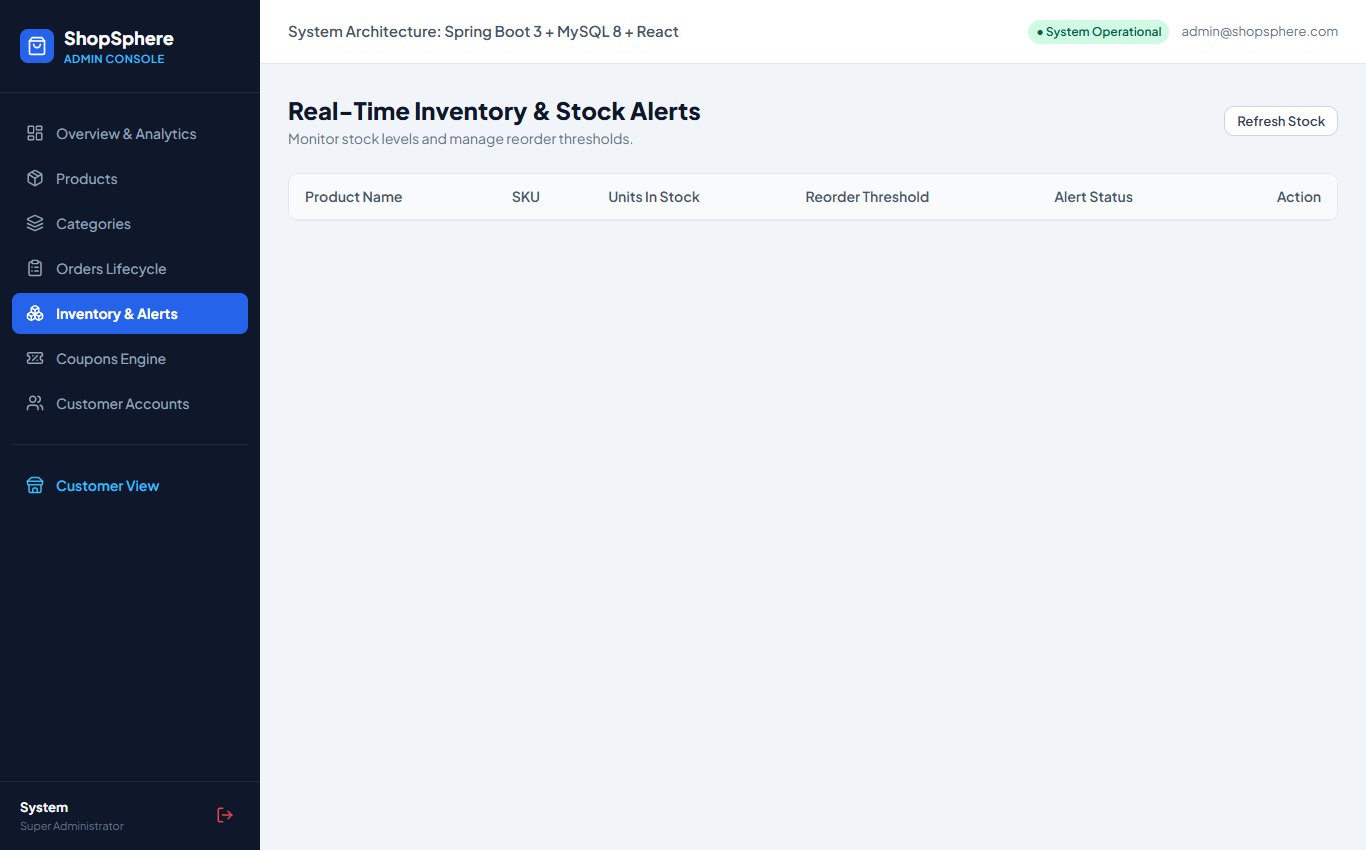
\includegraphics[width=0.96\textwidth]{09_admin_inventory.png}}
\caption{Live Output: Admin Low-Stock Sentinel and Warehouse Inventory Monitor}
\label{fig:screen_admin_inv}
\end{figure}
